\chapter{Presentaciones y Pruebas del Prototipo}\label{ch:Pruebas}
A lo largo del año de desarrollo, el prototipo del simulador fue presentado en diversos eventos e instituciones, lo que permitió recopilar retroalimentación clave para optimizar su funcionalidad y experiencia de usuario. Además, estas pruebas y presentaciones sirvieron para validar la precisión química de las reacciones y procesos representados, en colaboración con especialistas en el área.

\section{Presentaciones Institucionales}
El simulador fue exhibido como parte de las actividades de difusión del \textbf{Centro de Innovación y Desarrollo Tecnológico (CIDETEC) del Instituto Politécnico Nacional (IPN)}. Estas presentaciones estuvieron dirigidas a grupos invitados de diversas universidades e instituciones educativas, que tuvieron la oportunidad de observar y probar el prototipo. Entre las instituciones participantes se encuentran:
\begin{itemize}
    \item Tecnológico de Estudios Superiores de Jocotitlán\\
    Fecha: 24 de mayo de 2024.
    \item ESIME-Culhuacán, IPN\\
    Fecha: 7 de junio de 2024.
    \item UPIIZ, IPN\\
    Fechas: 21 de junio de 2024 y 27 de septiembre de 2024.
    \item Universidad Tecnológica de Xicotepec de Juárez\\
    Fecha: 5 de julio de 2024.
    \item Universidad Mexiquense del Bicentenario\\
    Fecha: 18 de octubre de 2024.
\end{itemize}
\begin{figure}[thbp]
    \centering
    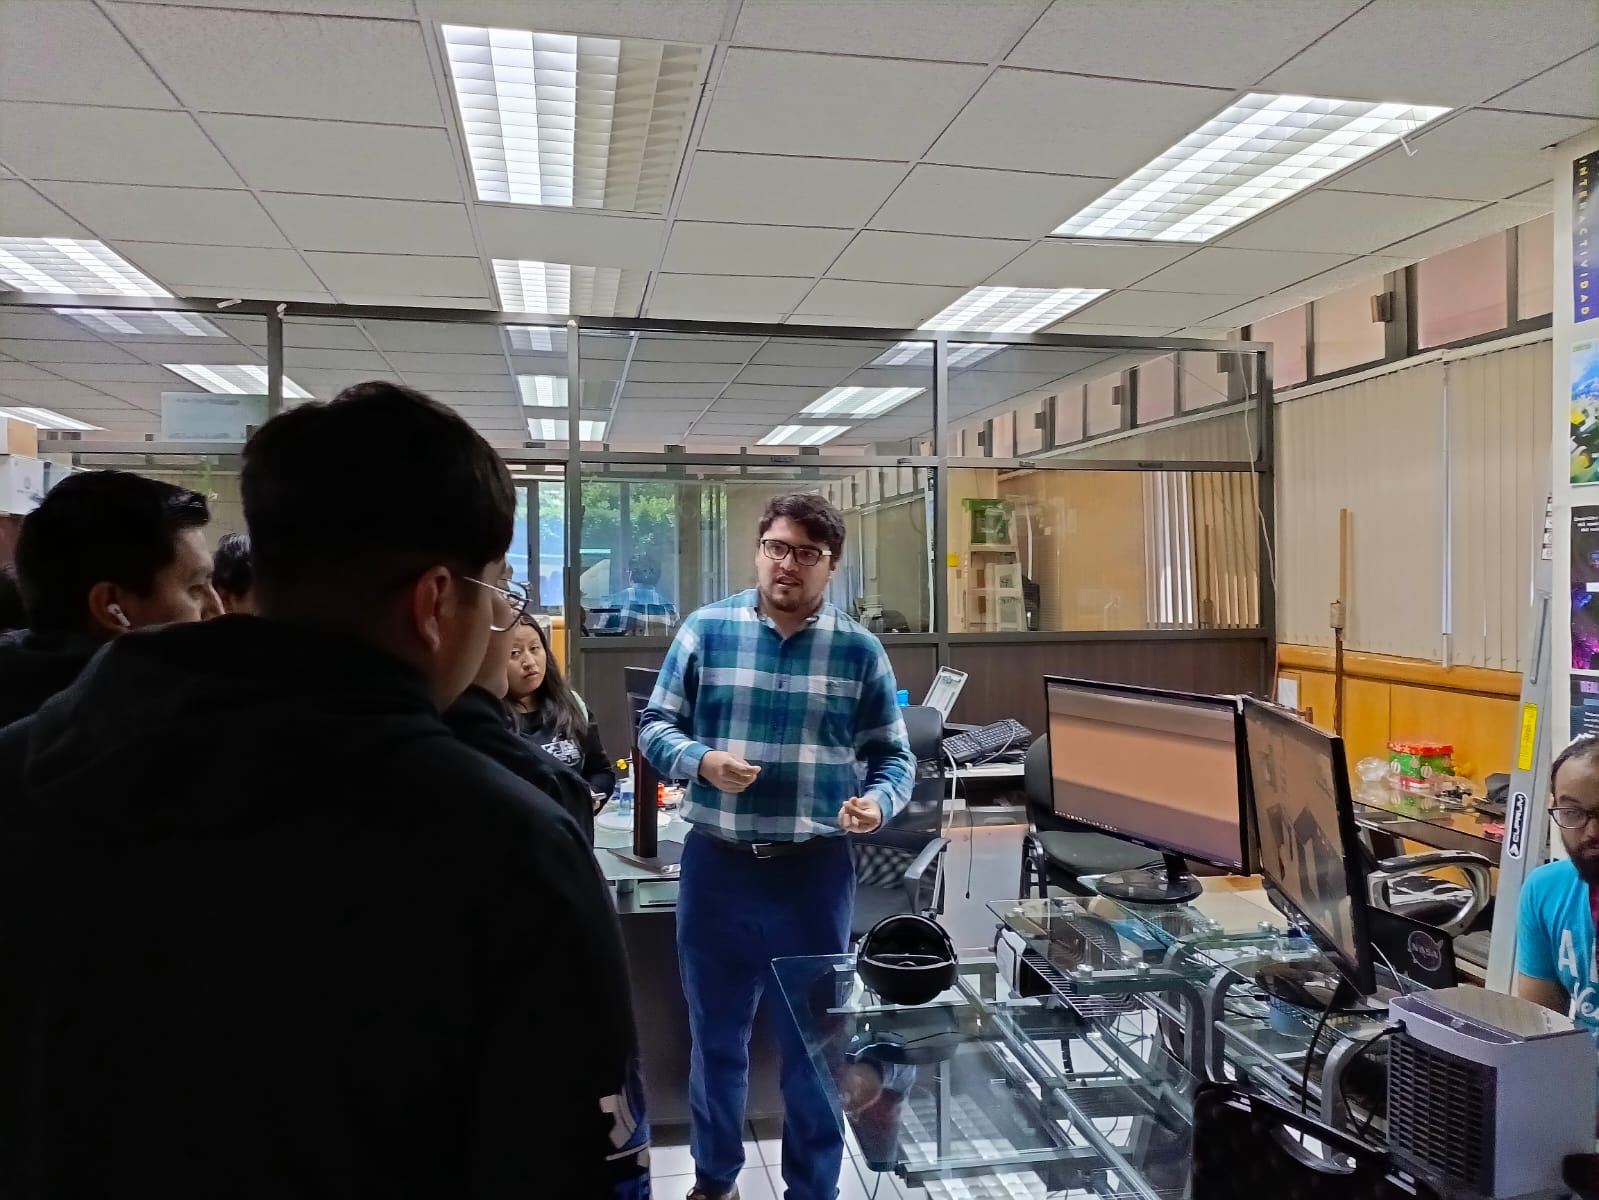
\includegraphics[width=0.7\textwidth, height = 7cm]{img/chapter06/CIDETEC.jpg}
    \caption{Presentaciones Institucionales}
    \label{fig:CIDETEC}
\end{figure}
Estas presentaciones permitieron recopilar observaciones de estudiantes en un entorno controlado, ayudando a identificar oportunidades de mejora y ajustar detalles técnicos del simulador.
\newline
\section{Invitaciones Externas}
Además de las presentaciones institucionales, el simulador fue invitado a participar en eventos externos y actividades organizadas por otras instituciones. Estas invitaciones ampliaron el alcance del proyecto y permitieron recibir retroalimentación de públicos diversos. Los eventos destacados incluyen:
\begin{itemize}
    \item \textbf{Centro de Estudios Superiores Isidro Fabela (Bachillerato)}\\
    Fecha: 13 de junio de 2024.
    \begin{figure}[thbp]
        \centering
        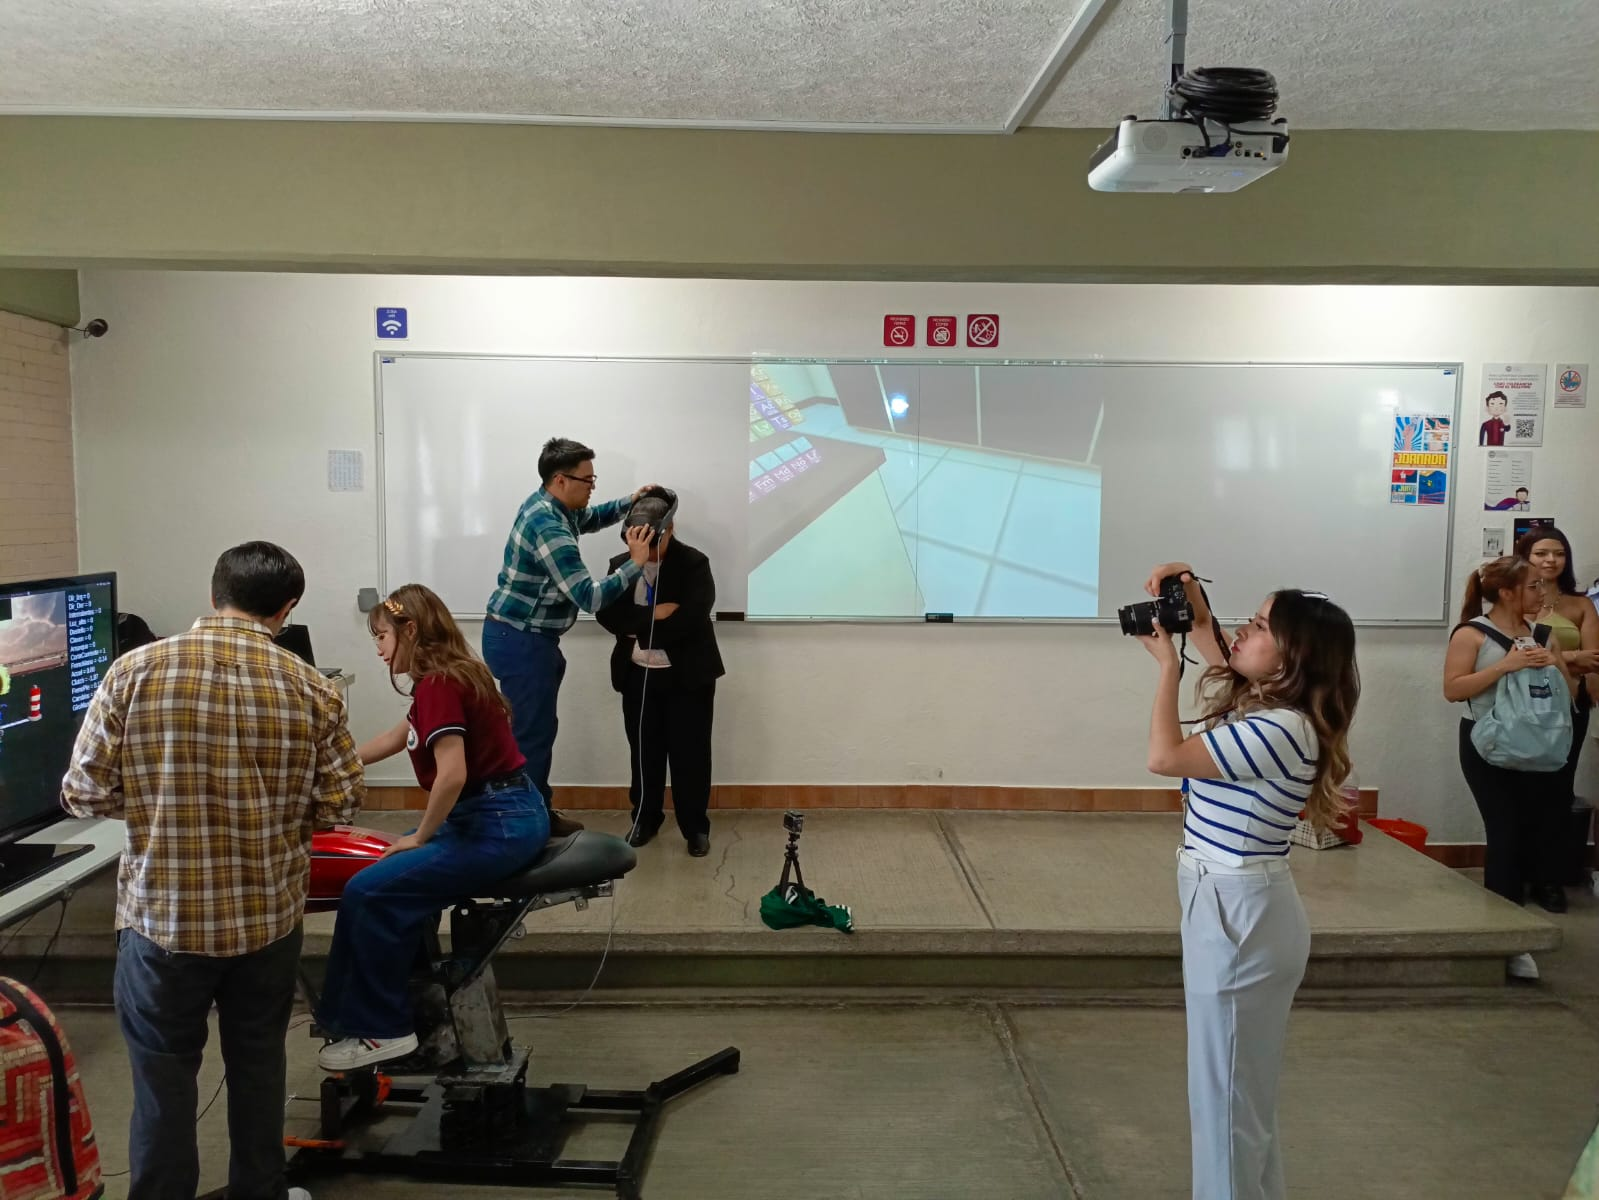
\includegraphics[width=0.5\textwidth, height = 5cm]{img/chapter06/CESIF_01.jpg}
        \caption{Presentación Isidro Fabela}
        \label{fig:CESIF}
    \end{figure}
    \newpage
    \item \textbf{Cinvesniños, CINVESTAV - IPN}\\
    Fechas: 22 y 23 de noviembre de 2024, en el stand  ``Uso de la realidad virtual en la ciencia''. Este fue el único evento público abierto, en el que participaron niños, jóvenes y adultos, ofreciendo perspectivas variadas sobre la accesibilidad y el impacto educativo del simulador.
    \begin{figure}[thbp]
        \centering
        \begin{subfigure}{0.45\linewidth}
            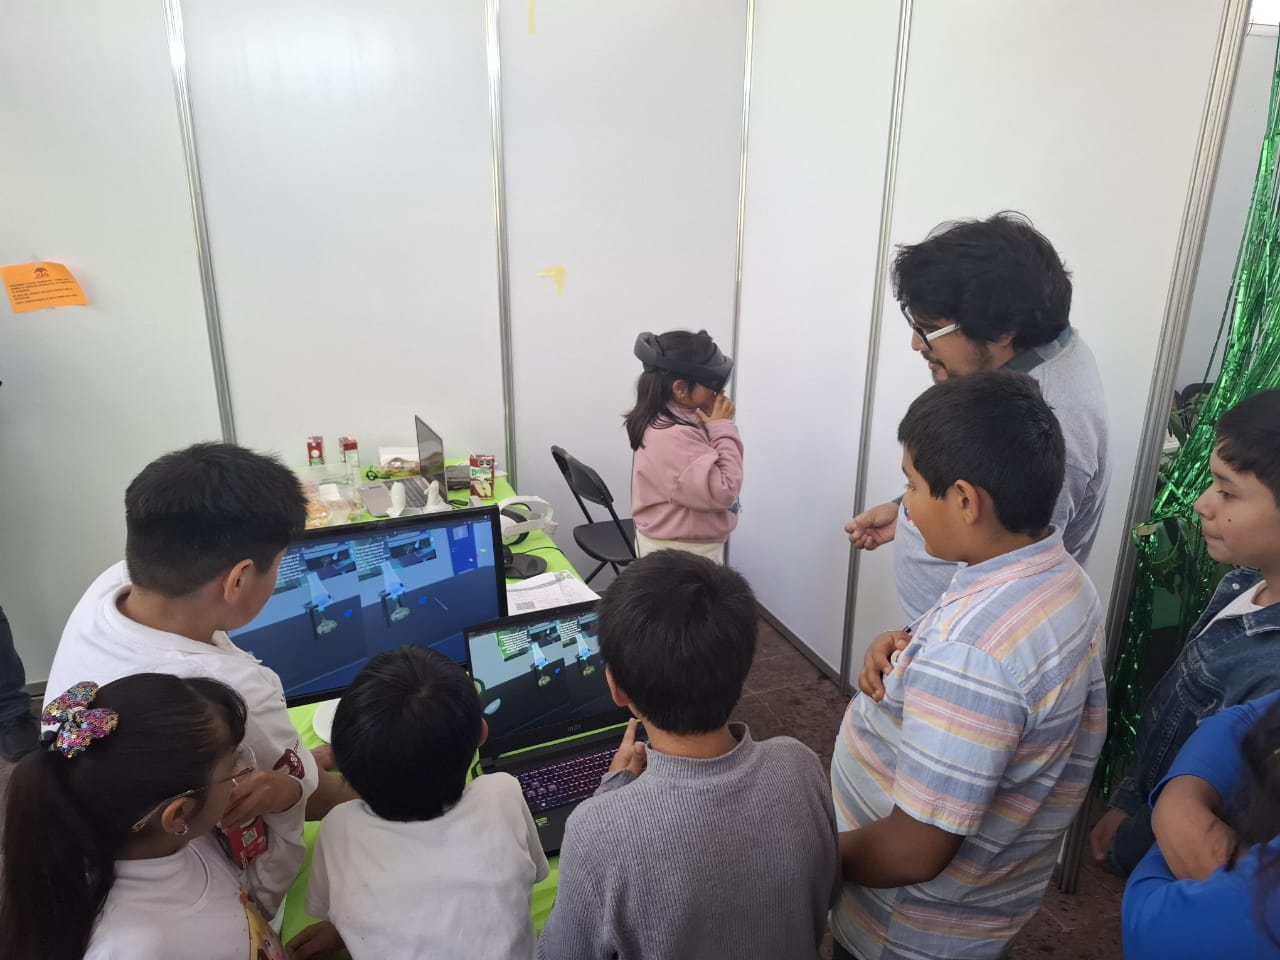
\includegraphics[width=\linewidth, height = 5cm]{img/chapter06/CINVESTAV_02.jpg}
        \end{subfigure}
        \begin{subfigure}{0.45\linewidth}
            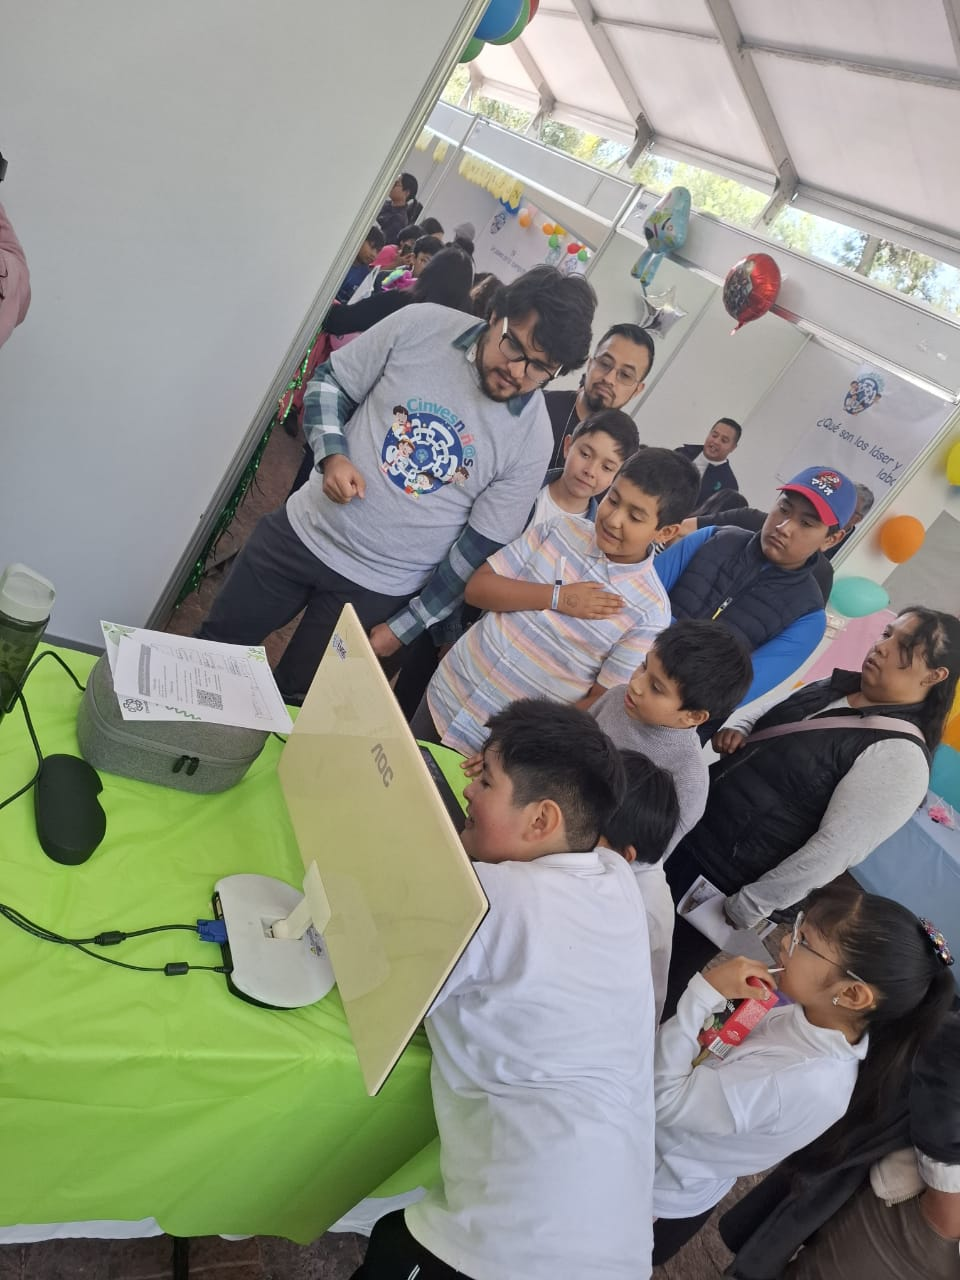
\includegraphics[width=\linewidth, height = 5cm]{img/chapter06/CINVESTAV_03.jpg}
        \end{subfigure}
        \caption{Presentación en Cinvesniños}
    \end{figure}
    \item \textbf{Universidad Estatal del Valle de Ecatepec}\\
    Fecha: 27 de noviembre de 2024.
    \begin{figure}[thbp]
        \centering
        \begin{subfigure}{0.45\linewidth}
            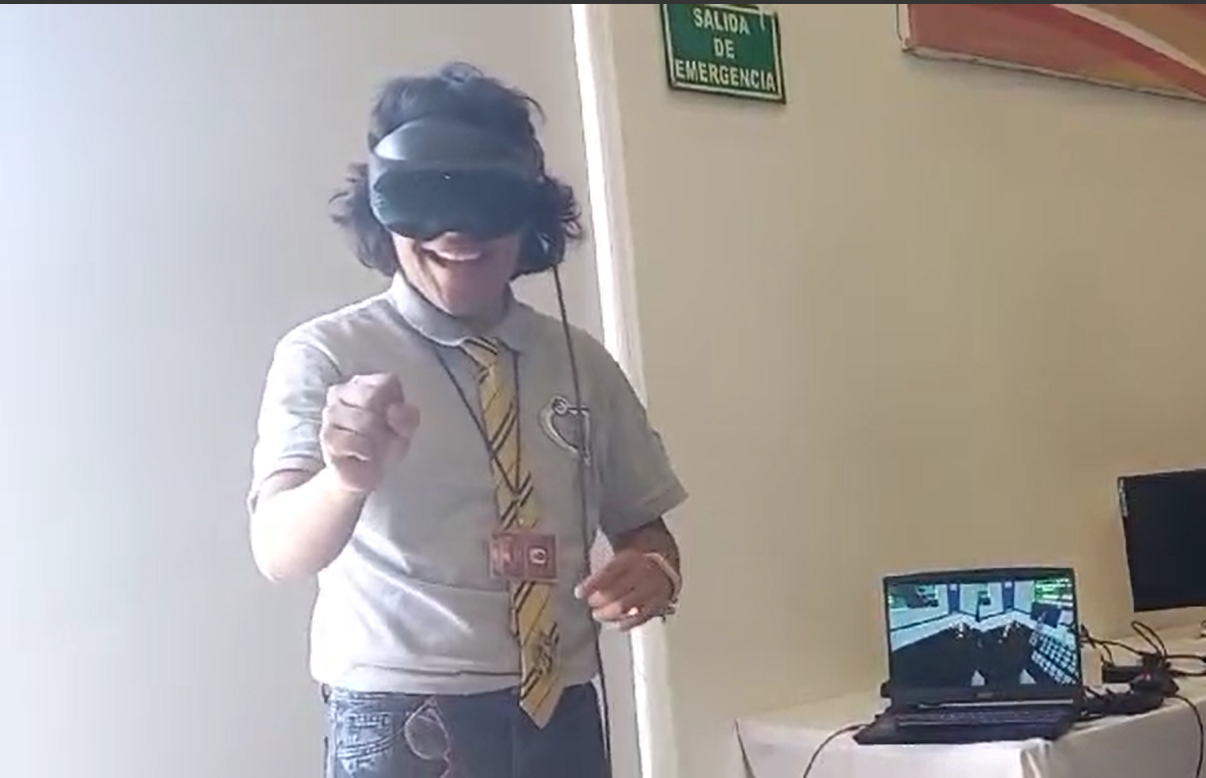
\includegraphics[width=\linewidth, height = 5cm]{img/chapter06/UEVE.png}
        \end{subfigure}
        \begin{subfigure}{0.45\linewidth}
            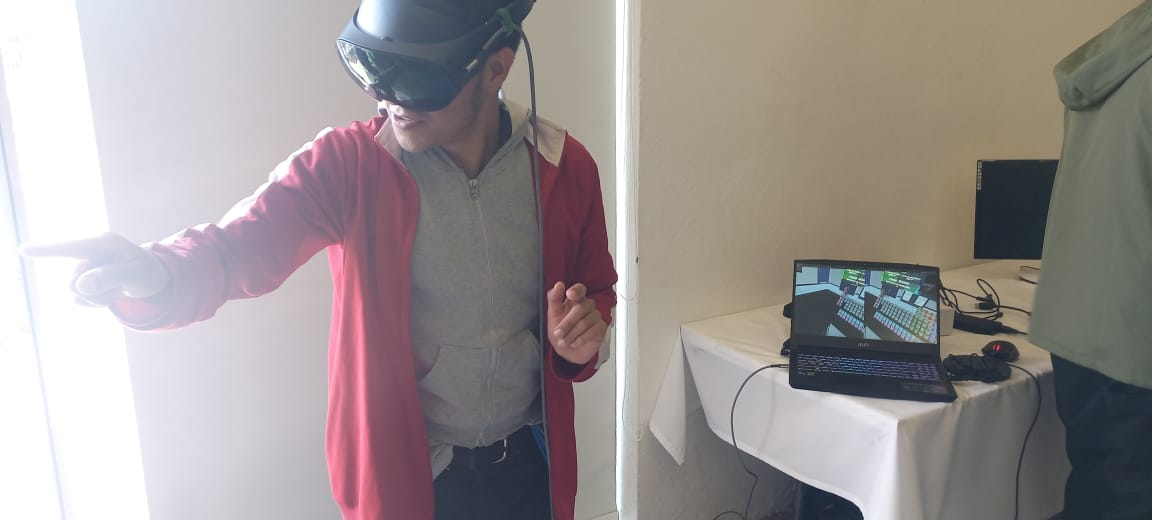
\includegraphics[width=\linewidth, height = 5cm]{img/chapter06/UEVE.jpg}
        \end{subfigure}
        \caption{Presentación UEVE}
    \end{figure}
\end{itemize}
\newpage
\section{Colaboración y Validación Académica}
Durante el desarrollo del proyecto, se contó con el apoyo de la Escuela Secundaria Diurna No. 4 ``Moisés Sáenz'' y del profesor Ernesto Uribe. Este trabajo conjunto incluyó sesiones de prueba con estudiantes y reuniones privadas para afinar detalles técnicos y validar la precisión de las reacciones químicas y los procesos educativos mostrados en el simulador.

Las pruebas realizadas con los estudiantes ayudaron a evaluar la usabilidad y la experiencia del usuario, mientras que las reuniones con el profesor permitieron garantizar la exactitud y la relevancia de la información química representada en el sistema.
\begin{figure}[thbp]
    \centering
    \begin{subfigure}{0.45\linewidth}
        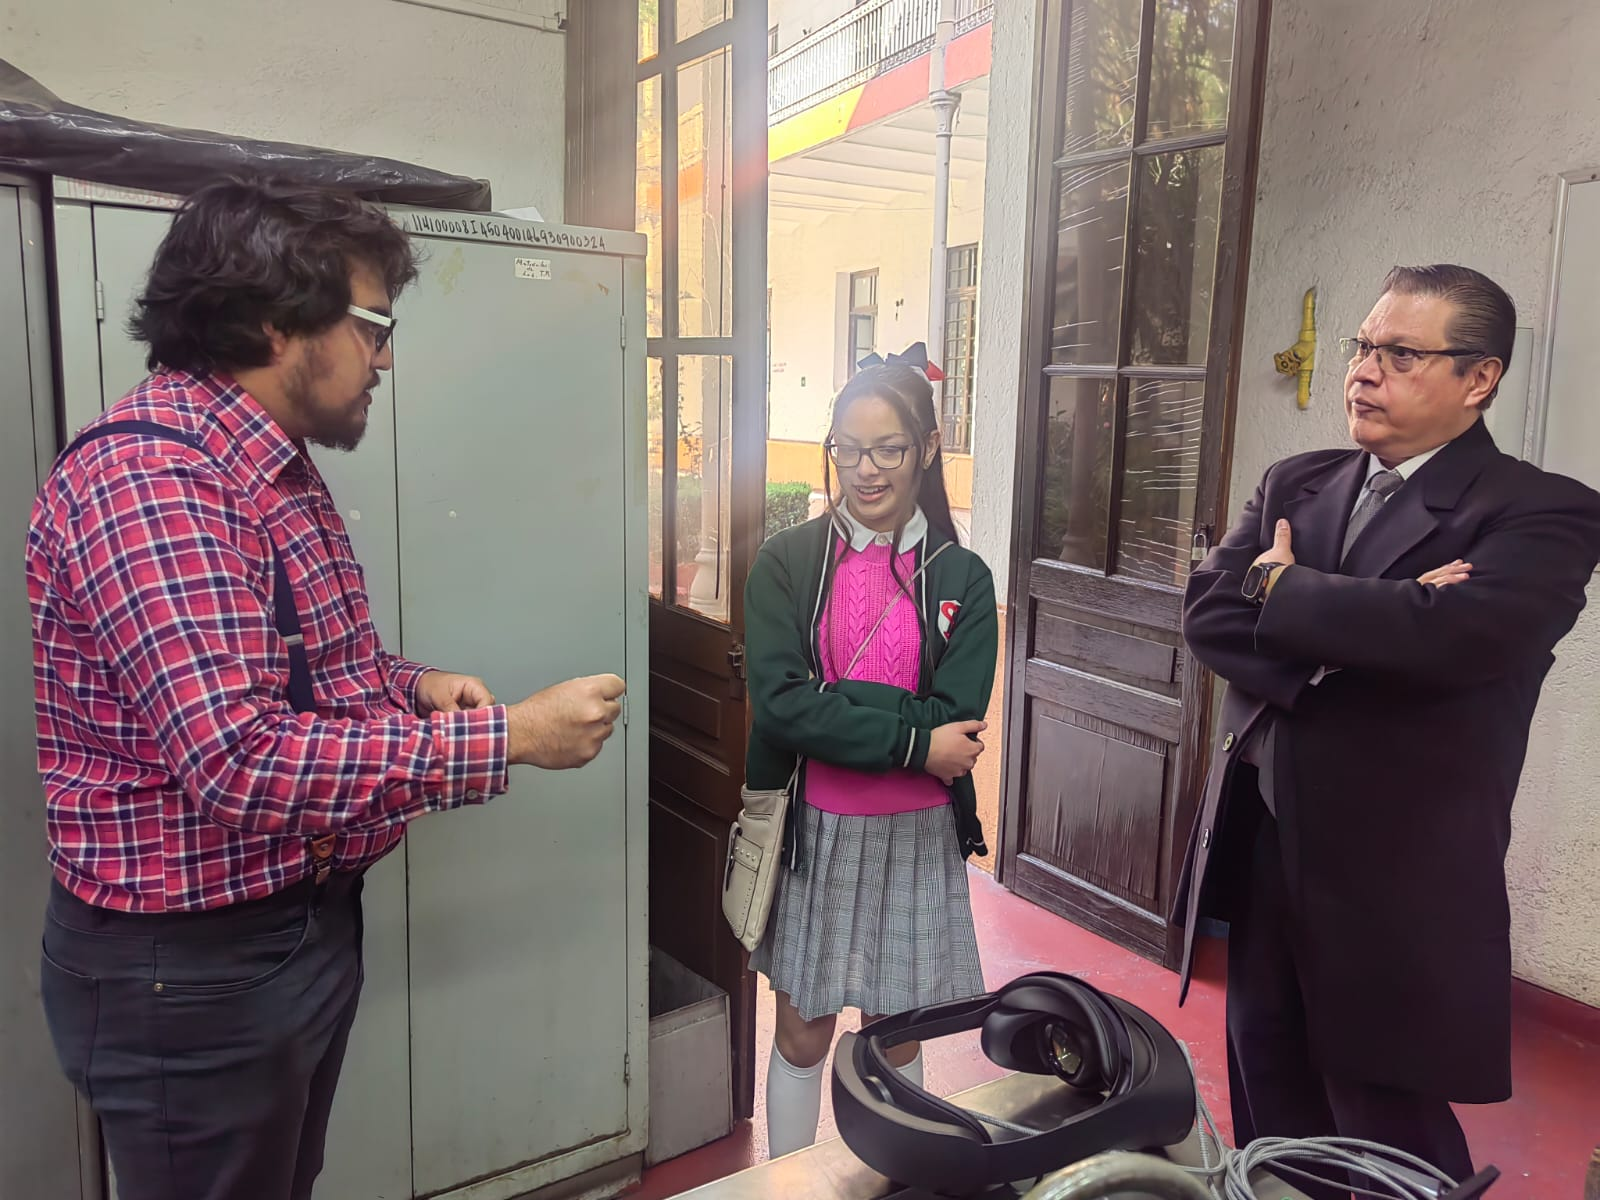
\includegraphics[width=\linewidth, height = 5cm]{img/chapter06/Sec_02.jpg}
    \end{subfigure}
    \begin{subfigure}{0.45\linewidth}
        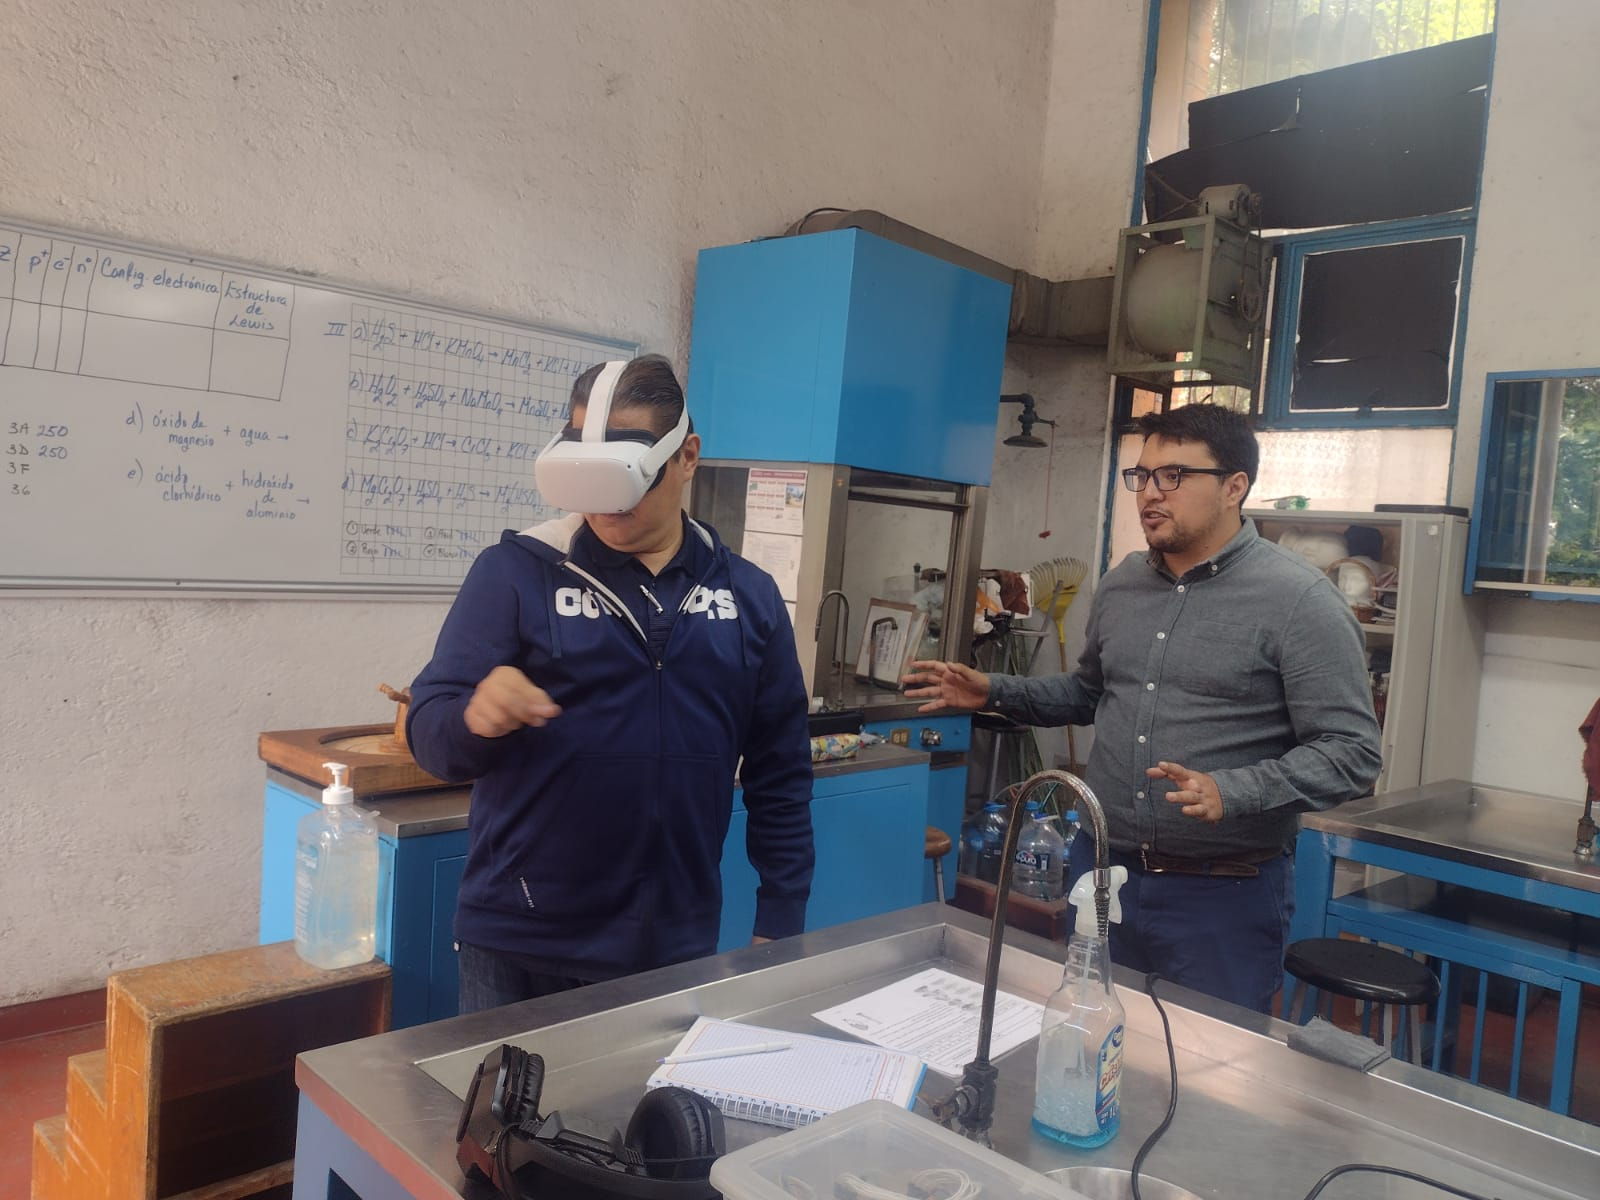
\includegraphics[width=\linewidth, height = 5cm]{img/chapter06/Sec_08.jpg}
    \end{subfigure}
    \begin{subfigure}{0.45\linewidth}
        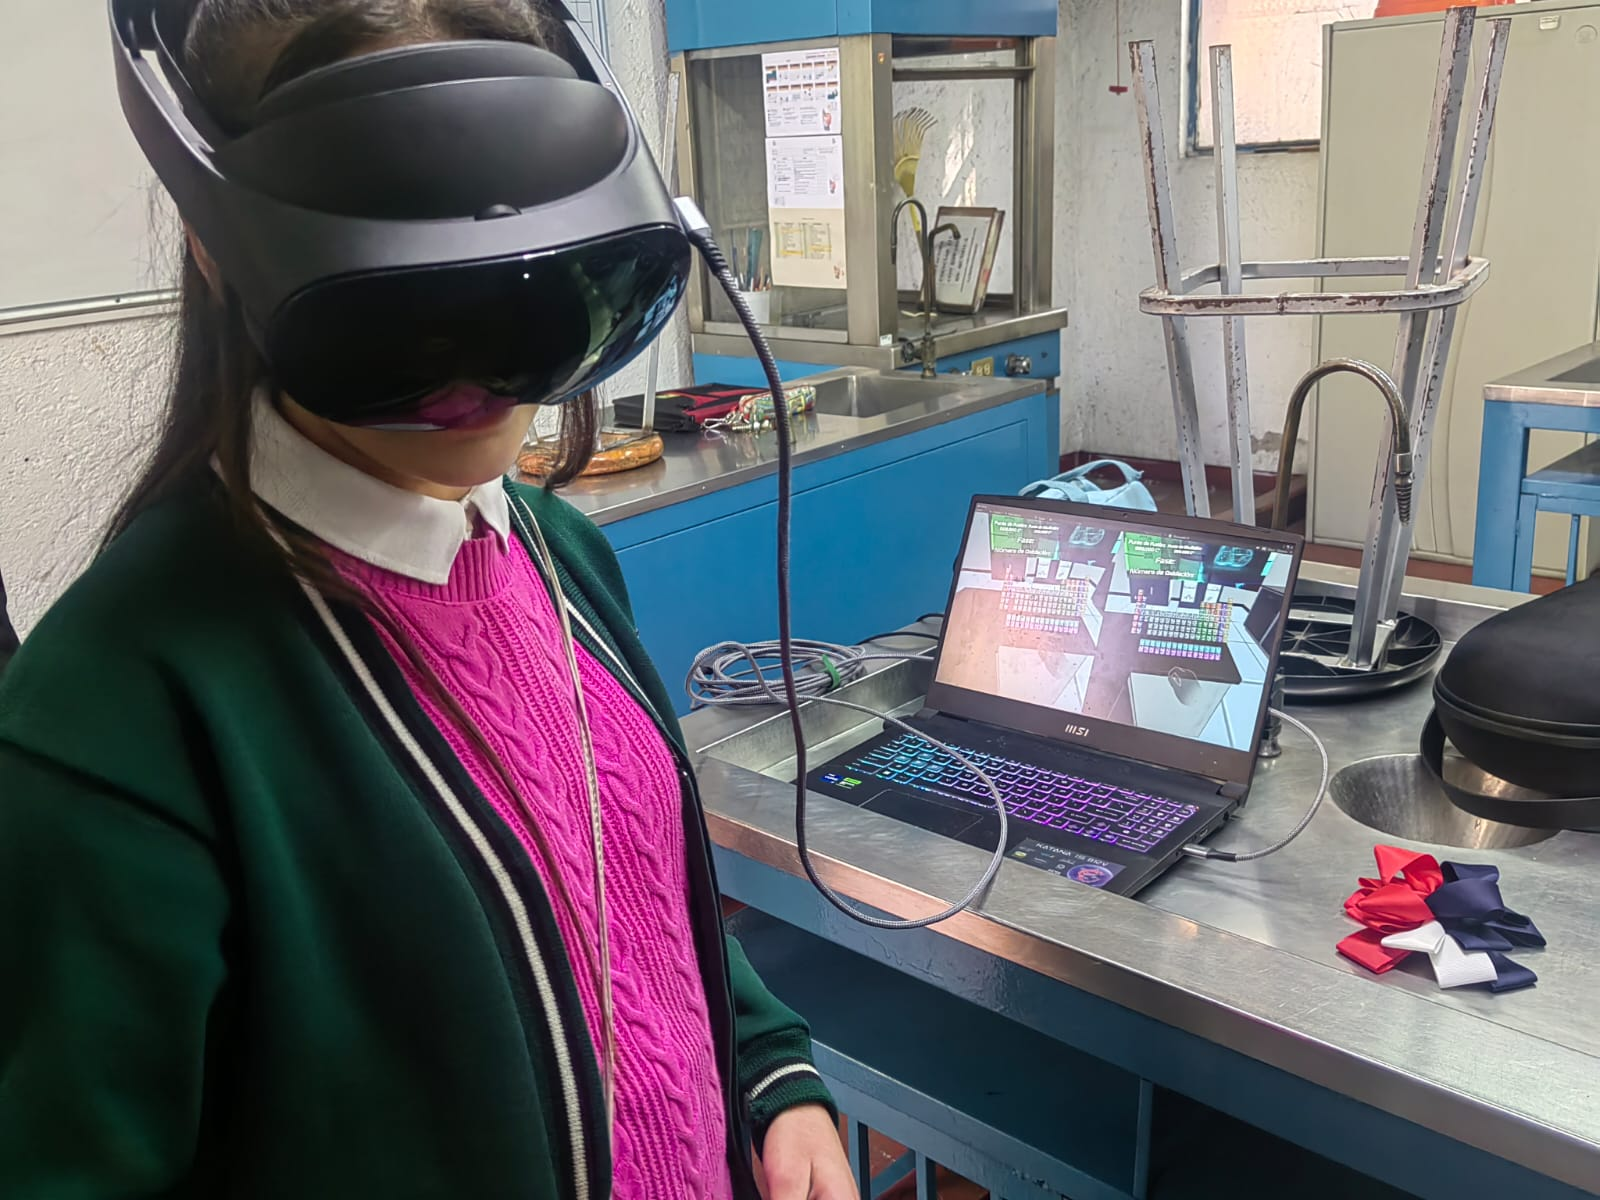
\includegraphics[width=\linewidth, height = 5cm]{img/chapter06/Sec_05.jpg}
    \end{subfigure}
    \caption{Reuniones en Secundaria 4}
\end{figure}